%========== Divide & Conquer ==========%

\chapter{Divide \& Conquer}
\label{ch:divideandconquer}

\textbf{Pensum} 2.3 + 4 + 7 \cite{clrs} \\\\
\textbf{Assignments} 2-2 (counter example), 7-1 (quicksort)\\\\
\textbf{Algorithms} Merge sort, quicksort, fibonacci\\\\
\textbf{Keywords} Recurrences, master method
\vspace{1in}

\noindent Divide and conquer is a paradigm of algorithmic methodologies. It
takes a problem and \textit{divides} it into several smaller subproblems,
until it reaches a base case, which makes the algorithm \textit{bottom out},
or \textit{conquer} each of these subproblems. \textit{Combining} the
solutions of all of the subproblems then yields a correct solution to the
original problem.
\\\\
\noindent \textbf{Divide} the problem into a number of subproblems that are
smaller instances of the same problem.
\\\\
\noindent \textbf{Conquer} the subproblems by solving them recursively. If the
subproblem sizes are small enough, however, just solve the subproblems
trivially.
\\\\
\noindent \textbf{Combine} the solutions to the subproblems into the solution
for the original problem.
\\\\

\section{Solving Recurrences}
% p. 83-97, CLRS 
Divide and conquer algorithms give rise to recurrence naturally, because they
call themselves recursively. To analyze the complexity of any recursive
algorithm we must describe it mathematically as an equation or inequality.
\\\\
We do this using one of three methods.
\begin{description}
	\item \textbf{Recursion trees} describes the recursions by means of a
tree-structure, by which we can then either guess or argue the complexity.
	\item \textbf{Substitution} uses a guessed bound, which could have been
derived from a recursion tree, and then by mathematical induction proves this
bound.
	\item \textbf{Master method} provides formulae for recurrences of the form
$T(n) = a T(n/b) + f(n)$, where $a \geq 1$, $b > 1$ and $f(n)$ is a given
function.
\end{description}

\subsection{Recursion Trees}
% p. 88-92, CLRS
A recursion tree is a pictorial representation of an algorithms recursive
calls. That is, we simply draw the recursions as they occur in a
tree-structure, such that we may make a guess as to the complexity of an
algorithm.

\begin{figure}[h]
	\center
	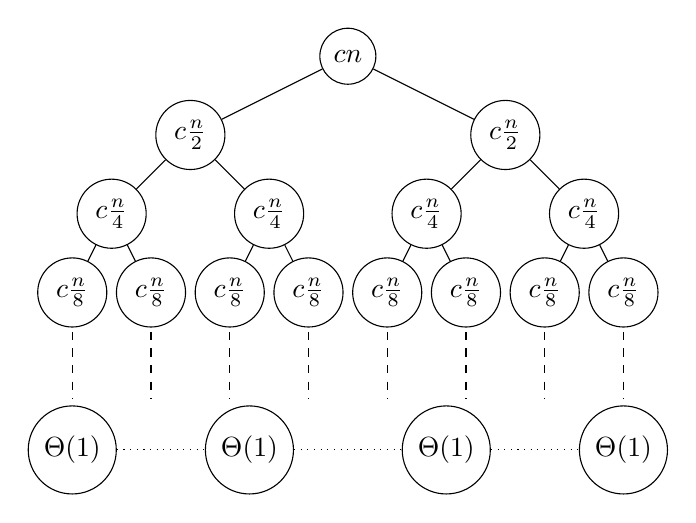
\begin{tikzpicture}
	[
	scale=1.0,
	align=center,
	every node/.style={circle, fill=white, draw=black}
	]
		% level 1
		\node (n1) at 	(3.5, -1) {$cn$};
		
		% level 2
		\node (n2) at 	(1.5, -2) {$c\frac{n}{2}$};
		\node (n3) at 	(5.5, -2) {$c\frac{n}{2}$};
		
		% level 3
		\node (n4) at 	(0.5, -3) {$c\frac{n}{4}$};
		\node (n5) at 	(2.5, -3) {$c\frac{n}{4}$};
		\node (n6) at 	(4.5, -3) {$c\frac{n}{4}$};
		\node (n7) at 	(6.5, -3) {$c\frac{n}{4}$};
		
		% level 4
		\node (n8) at 	(0, -4) {$c\frac{n}{8}$};
		\node (n9) at 	(1, -4) {$c\frac{n}{8}$};
		\node (n10) at 	(2, -4) {$c\frac{n}{8}$};
		\node (n11) at 	(3, -4) {$c\frac{n}{8}$};
		\node (n12) at 	(4, -4) {$c\frac{n}{8}$};
		\node (n13) at 	(5, -4) {$c\frac{n}{8}$};
		\node (n14) at 	(6, -4) {$c\frac{n}{8}$};
		\node (n15) at 	(7, -4) {$c\frac{n}{8}$};
		
		% bottom-out level
		\node (l1) at (0, -6) {$\Theta(1)$};
		\node (l2) at (2.25, -6) {$\Theta(1)$};
		\node (l3) at (4.75, -6) {$\Theta(1)$};
		\node (l4) at (7, -6) {$\Theta(1)$};
		
		% drawing code
		\draw [dashed] (0, -4.5) -- (0, -5.35);
		\draw [dashed] (1, -4.5) -- (1, -5.35);
		\draw [dashed] (2, -4.5) -- (2, -5.35);
		\draw [dashed] (3, -4.5) -- (3, -5.35);
		\draw [dashed] (4, -4.5) -- (4, -5.35);
		\draw [dashed] (5, -4.5) -- (5, -5.35);
		\draw [dashed] (6, -4.5) -- (6, -5.35);
		\draw [dashed] (7, -4.5) -- (7, -5.35);
		\foreach \from/\to in {n1/n2,n1/n3} \draw (\from) -- (\to);
		\foreach \from/\to in {n2/n4,n2/n5,n3/n6,n3/n7} \draw (\from) -- (\to);
		\foreach \from/\to in {n4/n8,n4/n9,n5/n10,n5/n11,n6/n12,n6/n13,n7/n14,n7/n15} \draw (\from) -- (\to);
		\foreach \from/\to in {l1/l2,l2/l3,l3/l4} \draw [dotted] (\from) -- (\to);
	\end{tikzpicture}

	\caption{Recurrence tree of merge sort.}
\end{figure}

Although recursion trees are useful for getting an idea about the complexity
of a recursive algorithm, it doesn't directly give us any concrete about this.
For that must employ more strict methods that are rooted in mathematics, and
not drawings - we can do this by induction with the substitution method (see
section \ref{ch:divideandconquer|sub:recurrences|subsub:substitution}).

\subsection{Substitution}
\label{ch:divideandconquer|sub:recurrences|subsub:substitution}
% p. 83-87, CLRS
The substitution method for solving recurrences consists of
two steps:
\begin{itemize}
\item Guess the form of the solution.
\item Use mathematical induction to find constants in the form and show that
the solution works.
\end{itemize}
The inductive hypothesis is applied to smaller values,
similar like recursive calls bring us closer to the base case
\\\\
\noindent \textbf{Example}\\
The recurrence relation for the cost of a divide-and-conquer method is
$T(n) = 2T( \lfloor n/2 \rfloor ) + n$. Our induction hypothesis of $T(n)$ is
$O(n \lg n)$ or $T(n) \leq cn \lg n$ for some constant $c$, independent of $n$.

Assume the hypothesis holds for all $m < n$ and substitute:
\begin{align}
	T(n) &\leq 2(c \lfloor n/2 \rfloor \lg_2 (\lfloor n/2 \rfloor )) + n \\
	&\leq cn \lg_2(n/2)+n \\
	&= cn \lg_2(n) - cn \lg_2(2)+n \\
	&= cn \lg_2(n) - cn + n \\
	&\leq cn \lg_2 (n)
\end{align}
as long as $c \geq 1$.

\newpage
\subsection{The Master Method}
\label{ch:divideandconquer|sub:recurrences|sub:master-theorem}
% p. 88-97, CLRS
For a divide-and-conquer algorithm $T(n)$, let $a$ denote the number of
subproblems created, and $n/b$ denote the size of each of these, on each
recursion. For each recursion we have a combine step, which takes $f(n)$.
We then have a recurrence of the form $T(n) = a T(n/b) + f(n)$.

Algorithms of this form can be solved by means of the master theorem, which
is given by
\begin{align}
\label{eqn:master-theorem}
	T(n) &= a T\left(\frac{n}{b}\right) + f(n)
	\begin{cases}
		f(n) = O(n^{\lg_b a - \epsilon}) & T(n) = \Theta(n^{\lg_b a}) \\
		f(n) = \Theta(n^{\lg_b a}) & T(n) = \Theta(n^{\lg_b a} \lg n) \\
		f(n) = O(n^{\lg_b a + \epsilon}) & * \Rightarrow T(n) = \Theta(f(n))
	\end{cases}
\end{align}
where $a \geq 1$, $b > 1$ and $\epsilon > 0$.
\begin{align}
	a f\left(\frac{n}{b}\right) &\leq c f(n)
	\text{, for all sufficiently large } n \text{, where } c < 1 \tag{*}
\end{align}
The first case $O(n^{\lg_b a - \epsilon})$ occurs when the \textit{divide}
step of the algorithm contributes the most to the complexity of the algorithm,
since $n^{\lg_b a} > f(n)$, and we therefore have to account for this by
subtracting $\epsilon$ from the exponent on the left-hand side. Vice versa for
the third case $O(n^{\lg_b a + \epsilon})$, which is symmetric. The second
case $\Theta(n^{\lg_b a})$ occurs when both steps, the \textit{divide} and
\textit{combine} step, are of the same complexity.
\\\\
\noindent \textbf{Example} \\
Consider the recurrence $T(n) = 2T(n/2) + f(n)$ of merge sort. We identify the
variables values as $a = 2$ since each recursive call creates two subproblems
and $b = 2$ since each of these are of $n/2$ the size of the previous problem.
The combine step is of linear time $\Theta(n)$.

We then have that $O(n^{\lg_2 2}) = f(n)$, since $f(n) = \Theta(n)$ and this
satisfies the previous equation, because $O(n^{\lg_2 2}) = \Theta(n)$.
Therefore, the second case of the master theorem applies to this algorithm,
and the complexity of it is then $\Theta(n^{lg_2 2}\lg n) = \Theta(n \lg n)$.

\newpage
\section{Quicksort}
The heart of this algorithm lies in the auxiliary procedure \texttt{Partition},
which rearranges the array in-place such that elements that are less than or
equal to a pivot are placed before it (lower index), and elements that are
greater than are placed after it (higher index).
\\\\
\noindent \textbf{Divide} the array $A[p \dots r]$ into two (possibly empty)
subarrays $A[p \dots q-1]$ and $A[q+1 \dots r]$ such that each element of the
former is less than $A[q]$, which is, in turn, less than or equal to each
element of the latter. Compute the index $q$ as part of this partitioning
procedure.
\\\\
\noindent \textbf{Conquer} the two subarrays by recursing.
\\\\
\noindent \textbf{Combine} isn't necessary, as the array is already sorted.

\subsection{Algorithm}
We give the algorithm (the initial call is
\texttt{QuickSort}($A$, 1, $A.length$). \\\\
\begin{algorithm}[H]
	\caption{Quick sort}
	\label{alg:quicksort}
	
	\SetKwInOut{In}{Input}
	\SetKwInOut{Out}{Output}
	
	\SetKwFunction{QuickSort}{QuickSort}
	\SetKwFunction{Partition}{Partition}
	
	\In{An unordered array $A$, start- and end-delimiting indices $p$ and $r$.}
	\Out{In-place reordering of the array $A$ in decreasing order.}
	
	\BlankLine
	
	\QuickSort($A$, $p$, $r$) \\
	\Begin
	{
		\If{$p < r$}
		{
			$q = $ \Partition($A$, $p$, $r$) \\
			\QuickSort($A$, $p$, $q-1$) \\
			\QuickSort($A$, $q+1$, $r$)
		}
	}
\end{algorithm}
And the partitioning procedure\\\\
\begin{algorithm}[H]
	\caption{Partition procedure}
	\label{alg:partition}
	
	\SetKwInOut{In}{Input}
	\SetKwInOut{Out}{Output}
	
	\SetKwFunction{Partition}{Partition}
	
	\In{An unordered array $A$, start- and end-delimiting indices $p$ and $r$.}
	\Out{In-place reordering of the array $A$ where all elements less than or
equal to the pivot has lower index that the pivot, likewise elements greater
than the pivot has a higher index. Returns the pivot index.}
	
	\BlankLine
	
	\Partition($A$, $p$, $r$) \\
	\Begin
	{
		$x = A[r]$ \\
		$i = p - 1$ \\
		\For{$j = p$ \KwTo $r - 1$}
		{
			\If{$A[j] \leq x$}
			{
				$i = i + 1$ \\
				Swap $A[i]$ with $A[j]$
			}
		}
		Swap $A[i + 1]$ with $A[r]$ \\
		\Return $i + 1$
	}
\end{algorithm}

\subsection{Proof}
% p. 173, CLRS
We state the loop invariant: at the beginning of each iteration of the
\texttt{for}-loop on lines 5-10, for any array index $k$, the following
holds
\begin{enumerate}
	\item If $p \leq k \leq i$, then $A[k] \leq x$.
	\item If $i + 1 \leq k \leq j - 1$, then $A[k] > x$.
	\item If $k = r$, then $A[k] = x$.
\end{enumerate}
\noindent \textbf{Initialization} Prior to the first iteration $i = p - 1$ and
$j = p$ no values lies between $p$ and $i$, and no values lies between $i + 1$
and $j - 1$, conditions 1 and 2 of the loop invariant are trivially
satisfied. The assignment on line 3 satisfies condition 3. \\
\\\\
\noindent \textbf{Maintenance} Two cases must be accounted for here because of
the \texttt{if}-statement on line 6; when $A[j] > x$, $j$ is incremented,
which then satisfies condition 2 for $A[j - 1]$, everything else remains
unchanged, thus satisfying conditions 1 and 3. When $A[j] \leq x$, then $i$ is
incremented and swap $A[i]$ and $A[j]$, and lastly increments $j$. Because of
the swap, we now have that $A[i] \leq q$, satisfying condition 1. Similarly,
we also have that $A[j - 1] > x$, since the item that was swapped into
$A[j - 1]$ is, by the loop invariant, greater than $x$.
\\\\
\noindent \textbf{Termination} At termination, $j = r$. Therefore, every entry
in the array is in one of the three sets described by the invariant, and the
partition is then in three parts; those less than or equal to $x$, those
greater than $x$ and a singleton set containing $x$.

\subsection{Analysis}
% p. 174-178, CLRS
The algorithm depends heavily on the partition subprocedure, and its
running-time is determined by the partition balance, which in turn depends on
the elements --- the more balanced, the faster it runs.
\\\\
\noindent \textbf{Worst-case partitioning} \\
The worst-case occurs when the partitioning subprocedure produces one
subproblem of size $n - 1$, and one with $0$ elements. Assuming that this
occurs on each recursive call, then the partitioning costs $\Theta(n)$. We
then have the recurrence
\begin{align}
	T(n) &= T(n-1) + T(0) + \Theta(n) \\ &= T(n-1) + \Theta(n) \\ &= \Theta(n^2)
\end{align}
Note that $T(n-1)$ forms an arithmetic series (see appendix
\ref{appendix:equations|eqn:arithmetic-series}), which evaluates to
$\Theta(n^2)$ --- which is just as slow as insertion sort.
\\\\
\noindent \textbf{Best-case partitioning} \\
The best-case occurs when the partition subprocedure splits the input in
evenly --- that is, sizes $\lfloor n/2 \rfloor$ and $\lceil n/2 \rceil - 1$.
We then have the recurrence
\begin{align}
	T(n) &= 2T(n/2) + \Theta(n)
\end{align}
By the master theorem (see section
\ref{ch:divideandconquer|sub:recurrences|sub:master-theorem}), this gives us a
running-time of $\Theta(n \lg n)$ --- which is just as fast as merge sort.

